% ================================================================
% EMPIRICAL APPLICATION — Dominick's Analgesics
% Auto-generated by run_dominicks_experiments.py
% n\_runs = 5  (mean $\pm$ std across independent re-estimations)
% Packages: booktabs, threeparttable, graphicx, siunitx
% ================================================================

\begin{table}[htbp]
  \centering
  \caption{Descriptive Statistics: Dominick's Analgesics Scanner Panel}
  \label{tab:dom_desc}
  \begin{threeparttable}
    \begin{tabular}{lS[table-format=2.3]S[table-format=1.3]S[table-format=1.4]S[table-format=1.4]}
      \toprule
      \textbf{Good} & {\textbf{Mean Price}} & {\textbf{Std Price}} & {\textbf{Mean Share}} & {\textbf{Std Share}} \\
      & {(\$/100 tablets)} & & & \\
      \midrule
      Aspirin & 7.311 & 1.557 & 0.2107 & 0.0519 \\
      Acetaminophen & 10.554 & 1.427 & 0.5026 & 0.0785 \\
      Ibuprofen & 10.506 & 1.428 & 0.2867 & 0.0819 \\
      \midrule
      \multicolumn{5}{l}{\textit{Train: 28,644 obs\quad Test: 4,287 obs\quad Stores: 93\quad Weeks: 1--399}} \\
      \bottomrule
    \end{tabular}
    \begin{tablenotes}\small
      \item Unit prices standardised to per-100-tablet equivalent.
    \end{tablenotes}
  \end{threeparttable}
\end{table}

\begin{table}[htbp]
  \centering
  \caption{Out-of-Sample Predictive Accuracy --- Dominick's Analgesics (5 independent re-estimations; mean $\pm$ std)}
  \label{tab:dom_acc}
  \begin{threeparttable}
    \begin{tabular}{lcc}
      \toprule
      \textbf{Model} & \textbf{RMSE} & \textbf{MAE} \\
      \midrule
      LA-AIDS & $0.07069 \pm 0.00000$ & $0.05593 \pm 0.00000$ \\
      Logit-IV & $0.07770 \pm 0.00000$ & $0.05992 \pm 0.00000$ \\
      QUAIDS & $0.06956 \pm 0.00000$ & $0.05519 \pm 0.00000$ \\
      Series Est. & $0.06514 \pm 0.00000$ & $0.05077 \pm 0.00000$ \\
      Neural Demand (window) & $0.04872 \pm 0.00008$ & $0.03662 \pm 0.00006$ \\
      Linear Demand (Shared) & $0.09201 \pm 0.00000$ & $0.07361 \pm 0.00000$ \\
      Linear Demand (GoodSpec) & $0.09197 \pm 0.00000$ & $0.07356 \pm 0.00000$ \\
      Linear Demand (Orth) & $0.08662 \pm 0.00000$ & $0.07046 \pm 0.00000$ \\
      Neural Demand (static) & $0.06477 \pm 0.00033$ & $0.05005 \pm 0.00025$ \\
      Neural Demand (habit) & $0.04766 \pm 0.00008$ & $0.03580 \pm 0.00010$ \\
      Neural Demand (FE) & $0.05880 \pm 0.00046$ & $0.04475 \pm 0.00046$ \\
      Neural Demand (habit, FE) & $0.04773 \pm 0.00004$ & $0.03585 \pm 0.00004$ \\
      Neural Demand (CF) & $0.06899 \pm 0.00046$ & $0.05266 \pm 0.00050$ \\
      \textbf{Neural Demand (habit, CF)} & \textbf{$0.04742 \pm 0.00004$} & $0.03572 \pm 0.00007$ \\
      Neural Demand (habit, FE, CF) & $0.04744 \pm 0.00014$ & $0.03568 \pm 0.00012$ \\
      PlaceboND & $0.06500 \pm 0.00047$ & $0.05017 \pm 0.00038$ \\
      \bottomrule
    \end{tabular}
    \begin{tablenotes}\small
      \item RMSE and MAE on held-out test observations, mean $\pm$ std over 5 run(s).
    \end{tablenotes}
  \end{threeparttable}
\end{table}

\begin{table}[htbp]
  \centering
  \caption{Own-Price Quantity Elasticities --- Dominick's Analgesics (5 run(s); mean $\pm$ std)}
  \label{tab:dom_elast}
  \begin{threeparttable}
    \begin{tabular}{lccc}
      \toprule
      \textbf{Model} & {$\hat{\varepsilon}_{00}$ (Aspirin)} & {$\hat{\varepsilon}_{11}$ (Acetaminophen)} & {$\hat{\varepsilon}_{22}$ (Ibuprofen)} \\
      \midrule
      LA-AIDS & $-0.849 \pm 0.000$ & $-1.420 \pm 0.000$ & $-1.140 \pm 0.000$ \\
      Logit-IV & $-0.999 \pm 0.000$ & $-1.770 \pm 0.000$ & $-0.586 \pm 0.000$ \\
      QUAIDS & $-0.882 \pm 0.000$ & $-1.423 \pm 0.000$ & $-1.129 \pm 0.000$ \\
      Series Est. & $-0.708 \pm 0.000$ & $-1.629 \pm 0.000$ & $-1.224 \pm 0.000$ \\
      Neural Demand (window) & $-0.979 \pm 0.008$ & $-1.188 \pm 0.005$ & $-1.435 \pm 0.011$ \\
      Linear Demand (Shared) & $-0.163 \pm 0.000$ & $-0.215 \pm 0.000$ & $-0.190 \pm 0.000$ \\
      Linear Demand (GoodSpec) & $-0.164 \pm 0.000$ & $-0.205 \pm 0.000$ & $-0.181 \pm 0.000$ \\
      Linear Demand (Orth) & $-1.165 \pm 0.000$ & $-1.125 \pm 0.000$ & $-1.177 \pm 0.000$ \\
      Neural Demand (static) & $-0.812 \pm 0.021$ & $-1.557 \pm 0.009$ & $-1.198 \pm 0.019$ \\
      Neural Demand (habit) & $-0.965 \pm 0.008$ & $-1.232 \pm 0.008$ & $-1.197 \pm 0.015$ \\
      Neural Demand (FE) & $-0.949 \pm 0.008$ & $-1.524 \pm 0.024$ & $-0.847 \pm 0.004$ \\
      Neural Demand (habit, FE) & $-0.953 \pm 0.007$ & $-1.253 \pm 0.008$ & $-1.179 \pm 0.013$ \\
      Neural Demand (CF) & $-0.923 \pm 0.023$ & $-1.659 \pm 0.038$ & $-0.779 \pm 0.034$ \\
      Neural Demand (habit, CF) & $-1.009 \pm 0.012$ & $-1.337 \pm 0.015$ & $-1.282 \pm 0.012$ \\
      Neural Demand (habit, FE, CF) & $-0.961 \pm 0.015$ & $-1.321 \pm 0.013$ & $-1.278 \pm 0.023$ \\
      PlaceboND & $-0.835 \pm 0.008$ & $-1.589 \pm 0.041$ & $-1.197 \pm 0.028$ \\
      \bottomrule
    \end{tabular}
    \begin{tablenotes}\small
      \item Numerical own-price quantity elasticities at mean test prices.
    \end{tablenotes}
  \end{threeparttable}
\end{table}

\begin{table}[htbp]
  \centering
  \caption{Consumer Surplus Loss from 10\% Ibuprofen Price Increase --- Dominick\'s Analgesics (5 run(s); mean $\pm$ std)}
  \label{tab:dom_welfare}
  \begin{threeparttable}
    \begin{tabular}{lcr}
      \toprule
      \textbf{Model} & \textbf{CV Loss (\$)} & \textbf{vs Neural Demand (static)} \\
      \midrule
      LA-AIDS & $-0.2322 \pm 0.0000$ & +1.0\% \\
      Logit-IV & $-0.2210 \pm 0.0000$ & +5.8\% \\
      QUAIDS & $-0.2339 \pm 0.0000$ & +0.3\% \\
      Series Est. & $-0.2333 \pm 0.0000$ & +0.5\% \\
      Neural Demand (window) & $-0.2379 \pm 0.0006$ & -1.4\% \\
      Linear Demand (Shared) & $-0.2823 \pm 0.0000$ & -20.4\% \\
      Linear Demand (GoodSpec) & $-0.2818 \pm 0.0000$ & -20.1\% \\
      Linear Demand (Orth) & $-0.2407 \pm 0.0000$ & -2.6\% \\
      Neural Demand (static) & $-0.2346 \pm 0.0011$ &  \\
      Neural Demand (habit) & $-0.2119 \pm 0.0012$ & +9.6\% \\
      Neural Demand (FE) & $-0.2420 \pm 0.0018$ & -3.2\% \\
      Neural Demand (habit, FE) & $-0.2166 \pm 0.0008$ & +7.7\% \\
      Neural Demand (CF) & $-0.2274 \pm 0.0016$ & +3.1\% \\
      Neural Demand (habit, CF) & $-0.2096 \pm 0.0007$ & +10.6\% \\
      Neural Demand (habit, FE, CF) & $-0.2169 \pm 0.0016$ & +7.5\% \\
      PlaceboND & $-0.2332 \pm 0.0009$ & +0.6\% \\
      \bottomrule
    \end{tabular}
    \begin{tablenotes}\small
      \item Compensating variation via 100-step Riemann sum, $p_{\mathrm{Ibu}}\to(1+0.1)\,p_{\mathrm{Ibu}}$.
    \end{tablenotes}
  \end{threeparttable}
\end{table}

\begin{table}[htbp]
  \centering
  \caption{Consumer Surplus Loss from 10\% Aspirin Price Increase --- Dominick\'s Analgesics (5 run(s); mean $\pm$ std)}
  \label{tab:dom_welfare_aspirin}
  \begin{threeparttable}
    \begin{tabular}{lcr}
      \toprule
      \textbf{Model} & \textbf{CV Loss (\$)} & \textbf{vs Neural Demand (static)} \\
      \midrule
      LA-AIDS & $-23.2182 \pm 0.0000$ & +1.0\% \\
      Logit-IV & $-22.1017 \pm 0.0000$ & +5.8\% \\
      QUAIDS & $-23.3916 \pm 0.0000$ & +0.3\% \\
      Series Est. & $-23.3300 \pm 0.0000$ & +0.5\% \\
      Neural Demand (window) & $-23.7881 \pm 0.0624$ & -1.4\% \\
      Linear Demand (Shared) & $-28.2325 \pm 0.0000$ & -20.4\% \\
      Linear Demand (GoodSpec) & $-28.1783 \pm 0.0000$ & -20.1\% \\
      Linear Demand (Orth) & $-24.0706 \pm 0.0000$ & -2.6\% \\
      Neural Demand (static) & $-23.4574 \pm 0.1137$ &  \\
      Neural Demand (habit) & $-21.1947 \pm 0.1241$ & +9.6\% \\
      Neural Demand (FE) & $-24.1964 \pm 0.1807$ & -3.2\% \\
      Neural Demand (habit, FE) & $-21.6555 \pm 0.0802$ & +7.7\% \\
      Neural Demand (CF) & $-22.7354 \pm 0.1615$ & +3.1\% \\
      Neural Demand (habit, CF) & $-20.9609 \pm 0.0653$ & +10.6\% \\
      Neural Demand (habit, FE, CF) & $-21.6882 \pm 0.1555$ & +7.5\% \\
      PlaceboND & $-23.3215 \pm 0.0932$ & +0.6\% \\
      \bottomrule
    \end{tabular}
    \begin{tablenotes}\small
      \item Compensating variation via 100-step Riemann sum, $p_{Aspirin}\to(1+0.1)\,p_{Aspirin}$.
    \end{tablenotes}
  \end{threeparttable}
\end{table}

\begin{table}[htbp]
  \centering
  \caption{Consumer Surplus Loss from 10\% Acetaminophen Price Increase --- Dominick\'s Analgesics (5 run(s); mean $\pm$ std)}
  \label{tab:dom_welfare_acetaminophen}
  \begin{threeparttable}
    \begin{tabular}{lcr}
      \toprule
      \textbf{Model} & \textbf{CV Loss (\$)} & \textbf{vs Neural Demand (static)} \\
      \midrule
      LA-AIDS & $-53.2076 \pm 0.0000$ & -3.7\% \\
      Logit-IV & $-47.9597 \pm 0.0000$ & +6.5\% \\
      QUAIDS & $-52.9144 \pm 0.0000$ & -3.1\% \\
      Series Est. & $-51.2835 \pm 0.0000$ & +0.1\% \\
      Neural Demand (window) & $-56.8829 \pm 0.1236$ & -10.9\% \\
      Linear Demand (Shared) & $-46.4907 \pm 0.0000$ & +9.4\% \\
      Linear Demand (GoodSpec) & $-46.5685 \pm 0.0000$ & +9.2\% \\
      Linear Demand (Orth) & $-56.5144 \pm 0.0000$ & -10.1\% \\
      Neural Demand (static) & $-51.3112 \pm 0.1514$ &  \\
      Neural Demand (habit) & $-49.5932 \pm 0.0333$ & +3.3\% \\
      Neural Demand (FE) & $-49.4375 \pm 0.2171$ & +3.7\% \\
      Neural Demand (habit, FE) & $-49.0632 \pm 0.1071$ & +4.4\% \\
      Neural Demand (CF) & $-49.2784 \pm 0.2842$ & +4.0\% \\
      Neural Demand (habit, CF) & $-49.1784 \pm 0.1133$ & +4.2\% \\
      Neural Demand (habit, FE, CF) & $-49.0017 \pm 0.2083$ & +4.5\% \\
      PlaceboND & $-51.6129 \pm 0.3441$ & -0.6\% \\
      \bottomrule
    \end{tabular}
    \begin{tablenotes}\small
      \item Compensating variation via 100-step Riemann sum, $p_{Acetaminophen}\to(1+0.1)\,p_{Acetaminophen}$.
    \end{tablenotes}
  \end{threeparttable}
\end{table}

\begin{table}[htbp]
  \centering
  \caption{Consumer Surplus Loss from 10\% Ibuprofen Price Increase --- Dominick\'s Analgesics (5 run(s); mean $\pm$ std)}
  \label{tab:dom_welfare_ibuprofen}
  \begin{threeparttable}
    \begin{tabular}{lcr}
      \toprule
      \textbf{Model} & \textbf{CV Loss (\$)} & \textbf{vs Neural Demand (static)} \\
      \midrule
      LA-AIDS & $-34.8710 \pm 0.0000$ & +3.5\% \\
      Logit-IV & $-38.1360 \pm 0.0000$ & -5.5\% \\
      QUAIDS & $-34.9710 \pm 0.0000$ & +3.2\% \\
      Series Est. & $-36.1016 \pm 0.0000$ & +0.1\% \\
      Neural Demand (window) & $-30.6435 \pm 0.1739$ & +15.2\% \\
      Linear Demand (Shared) & $-42.1538 \pm 0.0000$ & -16.6\% \\
      Linear Demand (GoodSpec) & $-42.1721 \pm 0.0000$ & -16.7\% \\
      Linear Demand (Orth) & $-31.0624 \pm 0.0000$ & +14.1\% \\
      Neural Demand (static) & $-36.1409 \pm 0.1286$ &  \\
      Neural Demand (habit) & $-40.7571 \pm 0.1109$ & -12.8\% \\
      Neural Demand (FE) & $-37.8776 \pm 0.2331$ & -4.8\% \\
      Neural Demand (habit, FE) & $-40.8281 \pm 0.1227$ & -13.0\% \\
      Neural Demand (CF) & $-39.3226 \pm 0.2975$ & -8.8\% \\
      Neural Demand (habit, CF) & $-40.9362 \pm 0.0619$ & -13.3\% \\
      Neural Demand (habit, FE, CF) & $-40.4954 \pm 0.1641$ & -12.0\% \\
      PlaceboND & $-35.8445 \pm 0.2216$ & +0.8\% \\
      \bottomrule
    \end{tabular}
    \begin{tablenotes}\small
      \item Compensating variation via 100-step Riemann sum, $p_{Ibuprofen}\to(1+0.1)\,p_{Ibuprofen}$.
    \end{tablenotes}
  \end{threeparttable}
\end{table}

\begin{table}[htbp]
  \centering
  \caption{Compensating Variation Comparison: 10\% Aspirin Price Increase}
  \label{tab:combined_welfare_aspirin}
  \begin{threeparttable}
  \begin{tabular}{lccccc}
    \toprule
    & \multicolumn{2}{c}{\textbf{Within-Category Revenue (T1)}} & & \multicolumn{2}{c}{\textbf{Median HH Income (T2)}} \\
    \cmidrule(lr){2-3} \cmidrule(lr){5-6}
    \textbf{Model} & \textbf{CV (\$)} & \textbf{vs. Stat (\%)} & & \textbf{CV (\$)} & \textbf{vs. Stat (\%)} \\
    \midrule
    \multicolumn{2}{l}{\textit{Traditional Models}} & & & & \\
    LA-AIDS & $-23.2182$ & $+1.0\%$ & & $-24.9433$ & $-0.8\%$ \\
             & $(0.0000)$ & & & $(0.3380)$ & \\
    \addlinespace
    BLP (IV) & $-22.1017$ & $+5.8\%$ & & $-21.5012$ & $+13.1\%$ \\
             & $(0.0000)$ & & & $(0.3161)$ & \\
    \addlinespace
    QUAIDS & $-23.3916$ & $+0.3\%$ & & $-26.1438$ & $-5.6\%$ \\
             & $(0.0000)$ & & & $(0.8232)$ & \\
    \addlinespace
    \multicolumn{2}{l}{\textit{Semi/Non-parametric}} & & & & \\
    Series Est. & $-23.3300$ & $+0.5\%$ & & $-24.6289$ & $+0.5\%$ \\
             & $(0.0000)$ & & & $(0.2073)$ & \\
    \addlinespace
    \multicolumn{2}{l}{\textit{Neural Demand}} & & & & \\
    Window & $-23.7881$ & $-1.4\%$ & & $-25.0067$ & $-1.0\%$ \\
             & $(0.0624)$ & & & $(0.3263)$ & \\
    \addlinespace
    Static & $-23.4574$ & --- & & $-24.7532$ & --- \\
             & $(0.1137)$ & & & $(0.2116)$ & \\
    \addlinespace
    Habit & $-21.1947$ & $+9.6\%$ & & $-22.6476$ & $+8.5\%$ \\
             & $(0.1241)$ & & & $(0.4710)$ & \\
             & \small{[$-21.35$, $-20.94$]} & & & \small{[$-22.18$, $-21.98$]} & \\
    \addlinespace
    FE & $-24.1964$ & $-3.2\%$ & & $-24.9081$ & $-0.6\%$ \\
             & $(0.1807)$ & & & $(0.3860)$ & \\
    \addlinespace
    Habit, FE & $-21.6555$ & $+7.7\%$ & & $-22.7915$ & $+7.9\%$ \\
             & $(0.0802)$ & & & $(0.4408)$ & \\
             & \small{[$-22.08$, $-21.48$]} & & & \small{[$-23.18$, $-22.64$]} & \\
    \addlinespace
    CF & $-22.7354$ & $+3.1\%$ & & $-23.6236$ & $+4.6\%$ \\
             & $(0.1615)$ & & & $(0.2803)$ & \\
    \addlinespace
    Habit, CF & $-20.9609$ & $+10.6\%$ & & $-22.5675$ & $+8.8\%$ \\
             & $(0.0653)$ & & & $(0.4568)$ & \\
             & \small{[$-21.24$, $-20.91$]} & & & \small{[$-22.17$, $-21.98$]} & \\
    \addlinespace
    Habit, FE, CF & $-21.6882$ & $+7.5\%$ & & $-22.7218$ & $+8.2\%$ \\
             & $(0.1555)$ & & & $(0.4419)$ & \\
             & \small{[$-21.97$, $-21.49$]} & & & \small{[$-23.06$, $-22.71$]} & \\
    \addlinespace
    Placebo & $-23.3215$ & $+0.6\%$ & & $-24.8101$ & $-0.2\%$ \\
             & $(0.0932)$ & & & $(0.2095)$ & \\
    \addlinespace
    \bottomrule
    \addlinespace
  \end{tabular}
  \begin{tablenotes}\small
    \item Mean CV with standard errors in parentheses. T1 uses total within-category analgesic revenue (hundreds of dollars) at mean test prices; this proxy is endogenous to the price shock. T2 retrains all models using store-level median household income from census-matched demographics as the budget variable (scaled to match within-category expenditure units); T2 standard errors are cluster-robust by store. 100-step Riemann sum, $p_{\mathrm{ASP}}\to1.10\,p_{\mathrm{ASP}}.$ Bracketed rows for habit models show the range of CV losses as the habit-decay parameter $\delta$ varies over the KL-identified set (test-KL within $2\times$ the standard error of the minimum in the fixed-$\delta$ grid; see the $\delta$ identification table). ``vs.\ Stat is per column relative to Neural Demand (static).
  \end{tablenotes}
  \end{threeparttable}
\end{table}

\begin{table}[htbp]
  \centering
  \caption{Compensating Variation Comparison: 10\% Acetaminophen Price Increase}
  \label{tab:combined_welfare_acetaminophen}
  \begin{threeparttable}
  \begin{tabular}{lccccc}
    \toprule
    & \multicolumn{2}{c}{\textbf{Within-Category Revenue (T1)}} & & \multicolumn{2}{c}{\textbf{Median HH Income (T2)}} \\
    \cmidrule(lr){2-3} \cmidrule(lr){5-6}
    \textbf{Model} & \textbf{CV (\$)} & \textbf{vs. Stat (\%)} & & \textbf{CV (\$)} & \textbf{vs. Stat (\%)} \\
    \midrule
    \multicolumn{2}{l}{\textit{Traditional Models}} & & & & \\
    LA-AIDS & $-53.2076$ & $-3.7\%$ & & $-54.3956$ & $-1.4\%$ \\
             & $(0.0000)$ & & & $(0.8827)$ & \\
    \addlinespace
    BLP (IV) & $-47.9597$ & $+6.5\%$ & & $-47.1434$ & $+12.1\%$ \\
             & $(0.0000)$ & & & $(0.6827)$ & \\
    \addlinespace
    QUAIDS & $-52.9144$ & $-3.1\%$ & & $-52.8934$ & $+1.4\%$ \\
             & $(0.0000)$ & & & $(0.3373)$ & \\
    \addlinespace
    \multicolumn{2}{l}{\textit{Semi/Non-parametric}} & & & & \\
    Series Est. & $-51.2835$ & $+0.1\%$ & & $-52.4159$ & $+2.2\%$ \\
             & $(0.0000)$ & & & $(0.4744)$ & \\
    \addlinespace
    \multicolumn{2}{l}{\textit{Neural Demand}} & & & & \\
    Window & $-56.8829$ & $-10.9\%$ & & $-59.3788$ & $-10.7\%$ \\
             & $(0.1236)$ & & & $(0.9029)$ & \\
    \addlinespace
    Static & $-51.3112$ & --- & & $-53.6194$ & --- \\
             & $(0.1514)$ & & & $(0.6805)$ & \\
    \addlinespace
    Habit & $-49.5932$ & $+3.3\%$ & & $-51.3093$ & $+4.3\%$ \\
             & $(0.0333)$ & & & $(0.8629)$ & \\
             & \small{[$-49.98$, $-49.27$]} & & & \small{[$-52.22$, $-51.51$]} & \\
    \addlinespace
    FE & $-49.4375$ & $+3.7\%$ & & $-54.2295$ & $-1.1\%$ \\
             & $(0.2171)$ & & & $(1.2587)$ & \\
    \addlinespace
    Habit, FE & $-49.0632$ & $+4.4\%$ & & $-51.2956$ & $+4.3\%$ \\
             & $(0.1071)$ & & & $(0.8718)$ & \\
             & \small{[$-49.37$, $-48.78$]} & & & \small{[$-51.23$, $-50.77$]} & \\
    \addlinespace
    CF & $-49.2784$ & $+4.0\%$ & & $-52.1045$ & $+2.8\%$ \\
             & $(0.2842)$ & & & $(0.8948)$ & \\
    \addlinespace
    Habit, CF & $-49.1784$ & $+4.2\%$ & & $-50.7489$ & $+5.4\%$ \\
             & $(0.1133)$ & & & $(0.8887)$ & \\
             & \small{[$-49.47$, $-48.79$]} & & & \small{[$-51.56$, $-51.14$]} & \\
    \addlinespace
    Habit, FE, CF & $-49.0017$ & $+4.5\%$ & & $-50.9372$ & $+5.0\%$ \\
             & $(0.2083)$ & & & $(0.9388)$ & \\
             & \small{[$-49.18$, $-48.60$]} & & & \small{[$-50.93$, $-50.68$]} & \\
    \addlinespace
    Placebo & $-51.6129$ & $-0.6\%$ & & $-53.9250$ & $-0.6\%$ \\
             & $(0.3441)$ & & & $(0.6380)$ & \\
    \addlinespace
    \bottomrule
    \addlinespace
  \end{tabular}
  \begin{tablenotes}\small
    \item Mean CV with standard errors in parentheses. T1 uses total within-category analgesic revenue (hundreds of dollars) at mean test prices; this proxy is endogenous to the price shock. T2 retrains all models using store-level median household income from census-matched demographics as the budget variable (scaled to match within-category expenditure units); T2 standard errors are cluster-robust by store. 100-step Riemann sum, $p_{\mathrm{ACET}}\to1.10\,p_{\mathrm{ACET}}.$ Bracketed rows for habit models show the range of CV losses as the habit-decay parameter $\delta$ varies over the KL-identified set (test-KL within $2\times$ the standard error of the minimum in the fixed-$\delta$ grid; see the $\delta$ identification table). ``vs.\ Stat is per column relative to Neural Demand (static).
  \end{tablenotes}
  \end{threeparttable}
\end{table}

\begin{table}[htbp]
  \centering
  \caption{Compensating Variation Comparison: 10\% Ibuprofen Price Increase}
  \label{tab:combined_welfare_ibuprofen}
  \begin{threeparttable}
  \begin{tabular}{lccccc}
    \toprule
    & \multicolumn{2}{c}{\textbf{Within-Category Revenue (T1)}} & & \multicolumn{2}{c}{\textbf{Median HH Income (T2)}} \\
    \cmidrule(lr){2-3} \cmidrule(lr){5-6}
    \textbf{Model} & \textbf{CV (\$)} & \textbf{vs. Stat (\%)} & & \textbf{CV (\$)} & \textbf{vs. Stat (\%)} \\
    \midrule
    \multicolumn{2}{l}{\textit{Traditional Models}} & & & & \\
    LA-AIDS & $-34.8710$ & $+3.5\%$ & & $-36.4478$ & $+2.1\%$ \\
             & $(0.0000)$ & & & $(0.5570)$ & \\
    \addlinespace
    BLP (IV) & $-38.1360$ & $-5.5\%$ & & $-37.8108$ & $-1.6\%$ \\
             & $(0.0000)$ & & & $(0.5690)$ & \\
    \addlinespace
    QUAIDS & $-34.9710$ & $+3.2\%$ & & $-36.7831$ & $+1.2\%$ \\
             & $(0.0000)$ & & & $(0.6648)$ & \\
    \addlinespace
    \multicolumn{2}{l}{\textit{Semi/Non-parametric}} & & & & \\
    Series Est. & $-36.1016$ & $+0.1\%$ & & $-38.2381$ & $-2.7\%$ \\
             & $(0.0000)$ & & & $(1.2498)$ & \\
    \addlinespace
    \multicolumn{2}{l}{\textit{Neural Demand}} & & & & \\
    Window & $-30.6435$ & $+15.2\%$ & & $-31.5028$ & $+15.4\%$ \\
             & $(0.1739)$ & & & $(0.5015)$ & \\
    \addlinespace
    Static & $-36.1409$ & --- & & $-37.2232$ & --- \\
             & $(0.1286)$ & & & $(0.8821)$ & \\
    \addlinespace
    Habit & $-40.7571$ & $-12.8\%$ & & $-42.3309$ & $-13.7\%$ \\
             & $(0.1109)$ & & & $(0.8813)$ & \\
             & \small{[$-41.30$, $-40.37$]} & & & \small{[$-42.69$, $-41.88$]} & \\
    \addlinespace
    FE & $-37.8776$ & $-4.8\%$ & & $-36.9756$ & $+0.7\%$ \\
             & $(0.2331)$ & & & $(0.6226)$ & \\
    \addlinespace
    Habit, FE & $-40.8281$ & $-13.0\%$ & & $-42.1938$ & $-13.4\%$ \\
             & $(0.1227)$ & & & $(0.8845)$ & \\
             & \small{[$-41.21$, $-40.18$]} & & & \small{[$-42.77$, $-41.91$]} & \\
    \addlinespace
    CF & $-39.3226$ & $-8.8\%$ & & $-40.2079$ & $-8.0\%$ \\
             & $(0.2975)$ & & & $(0.7179)$ & \\
    \addlinespace
    Habit, CF & $-40.9362$ & $-13.3\%$ & & $-42.4607$ & $-14.1\%$ \\
             & $(0.0619)$ & & & $(0.8418)$ & \\
             & \small{[$-41.37$, $-40.55$]} & & & \small{[$-42.52$, $-42.01$]} & \\
    \addlinespace
    Habit, FE, CF & $-40.4954$ & $-12.0\%$ & & $-42.1986$ & $-13.4\%$ \\
             & $(0.1641)$ & & & $(0.7899)$ & \\
             & \small{[$-40.92$, $-40.10$]} & & & \small{[$-42.34$, $-41.80$]} & \\
    \addlinespace
    Placebo & $-35.8445$ & $+0.8\%$ & & $-36.8859$ & $+0.9\%$ \\
             & $(0.2216)$ & & & $(0.9211)$ & \\
    \addlinespace
    \bottomrule
    \addlinespace
  \end{tabular}
  \begin{tablenotes}\small
    \item Mean CV with standard errors in parentheses. T1 uses total within-category analgesic revenue (hundreds of dollars) at mean test prices; this proxy is endogenous to the price shock. T2 retrains all models using store-level median household income from census-matched demographics as the budget variable (scaled to match within-category expenditure units); T2 standard errors are cluster-robust by store. 100-step Riemann sum, $p_{\mathrm{IBU}}\to1.10\,p_{\mathrm{IBU}}.$ Bracketed rows for habit models show the range of CV losses as the habit-decay parameter $\delta$ varies over the KL-identified set (test-KL within $2\times$ the standard error of the minimum in the fixed-$\delta$ grid; see the $\delta$ identification table). ``vs.\ Stat is per column relative to Neural Demand (static).
  \end{tablenotes}
  \end{threeparttable}
\end{table}

\begin{table}[htbp]
  \centering
  \caption{MDP State Augmentation: Brand Loyalty in Analgesic Demand (5 run(s); mean $\pm$ std)}
  \label{tab:dom_mdp}
  \begin{threeparttable}
    \begin{tabular}{lcccc}
      \toprule
      \textbf{Model} & \textbf{RMSE} & \textbf{KL Div.} & \textbf{Reduction} \\
      \midrule
      LA-AIDS & $0.07069 \pm 0.00000$ & $0.02311 \pm 0.00000$ & baseline \\
      Neural Demand (static) & $0.06477 \pm 0.00033$ & $0.01984 \pm 0.00019$ & 8.4% \\
      Neural Demand (habit) & $0.04766 \pm 0.00008$ & $0.01068 \pm 0.00003$ & 32.6% \\
      PlaceboND & $0.06500 \pm 0.00047$ & $0.01994 \pm 0.00026$ & 8.0% \\
      Neural Demand (CF) & $0.06899 \pm 0.00046$ & $0.02177 \pm 0.00031$ & 2.4% \\
      Neural Demand (habit, CF) & $0.04742 \pm 0.00004$ & $0.01058 \pm 0.00002$ & 32.9% \\
      \bottomrule
    \end{tabular}
    \begin{tablenotes}\small
      \item Habit-decay $\hat{\delta}$ (habit model) = 0.800$\pm$0.000; FE variant: 0.800$\pm$0.000.
      RMSE and KL: mean $\pm$ std over 5 independent re-estimation(s).
      \item \textbf{Diebold-Mariano Test}: Static vs Habit (blocked by store). DM stat = 8.09^{***} ($p=2.748e-12$). Positive stat favors Habit model.
    \end{tablenotes}
  \end{threeparttable}
\end{table}

\begin{table}[htbp]
  \centering
  \caption{Cross-Price Elasticity Matrix (Neural Demand (habit)) (5 run(s); mean $\pm$ std)}
  \label{tab:dom_cross_elast_table}
  \begin{threeparttable}
    \begin{tabular}{lccc}
      \toprule
      & \multicolumn{3}{c}{\textbf{Price of}} \\
      \cmidrule(lr){2-4}
      \textbf{Quantity of} & \textbf{Aspirin} & \textbf{Acetaminophen} & \textbf{Ibuprofen} \\
      \midrule
      Aspirin & \textbf{$-0.965 \pm 0.008$} & $-0.002 \pm 0.014$ & $-0.015 \pm 0.017$ \\
      Acetaminophen & $0.014 \pm 0.030$ & \textbf{$-1.232 \pm 0.008$} & $0.275 \pm 0.017$ \\
      Ibuprofen & $-0.003 \pm 0.016$ & $0.163 \pm 0.008$ & \textbf{$-1.197 \pm 0.015$} \\
      \bottomrule
    \end{tabular}
    \begin{tablenotes}\small
      \item Row $i$, Column $j$: $\epsilon_{ij} = \partial \log q_i / \partial \log p_j$.
      \item Evaluated at mean test prices. Mean $\pm$ std over runs.
    \end{tablenotes}
  \end{threeparttable}
\end{table}

\begin{figure}[htbp]
  \centering
  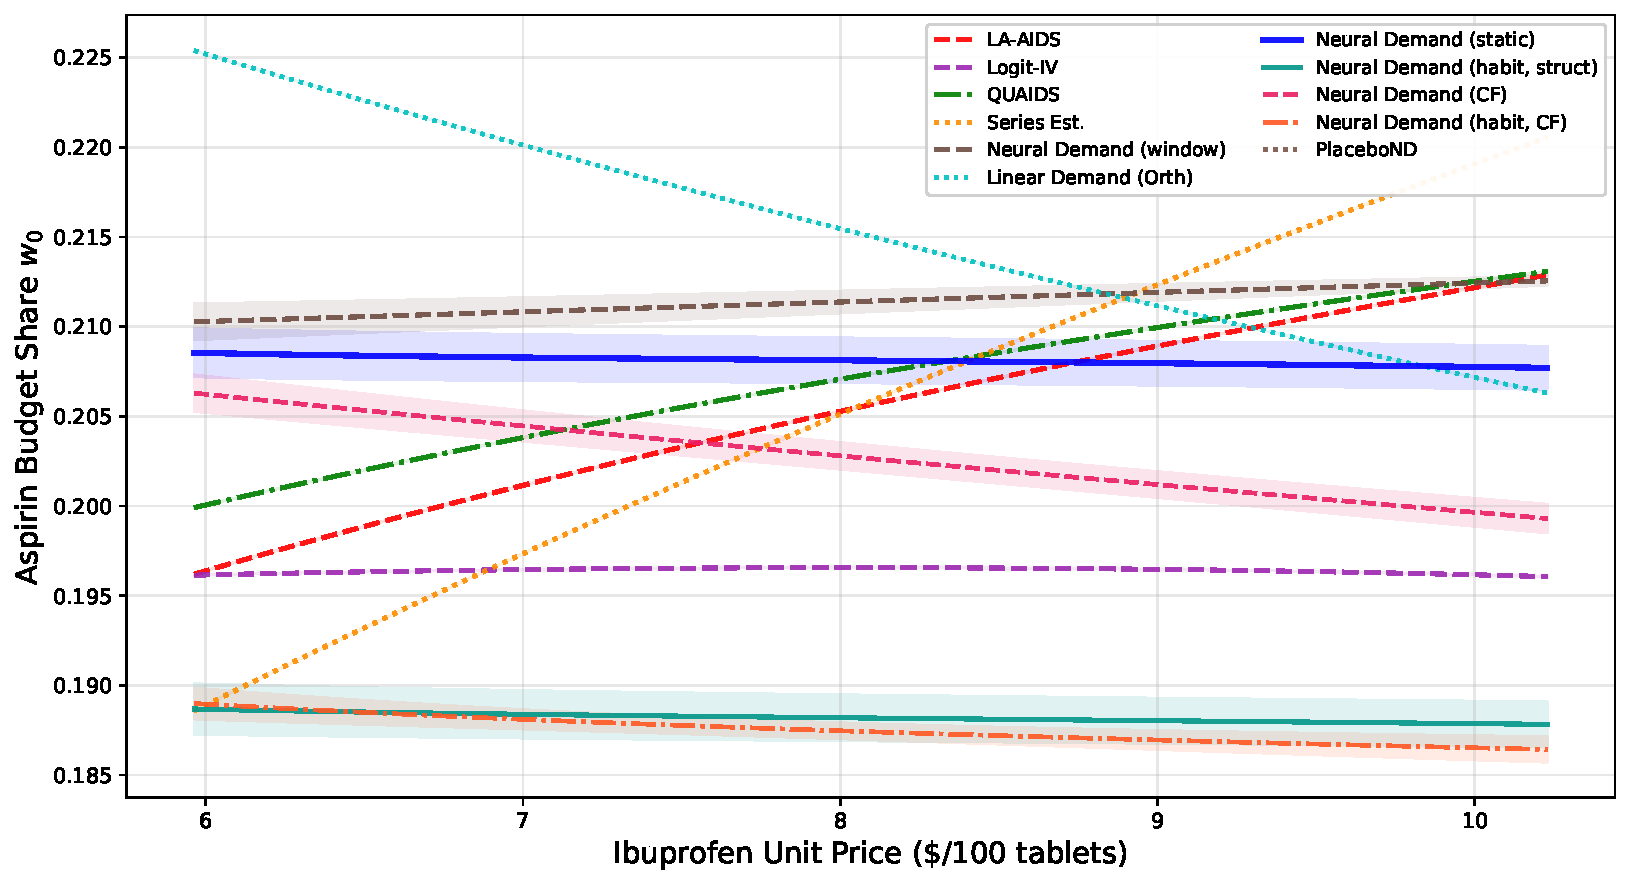
\includegraphics[width=\textwidth]{results/neural_demand/dominicks/figures/fig_demand_curves.pdf}
  \caption{Aspirin Budget Share as a Function of Ibuprofen Unit Price --- Dominick's Analgesics. Shaded bands indicate $\pm 1$ standard deviation across 5 independent re-estimations.}
  \label{fig:dom_demand}
\end{figure}

\begin{figure}[htbp]
  \centering
  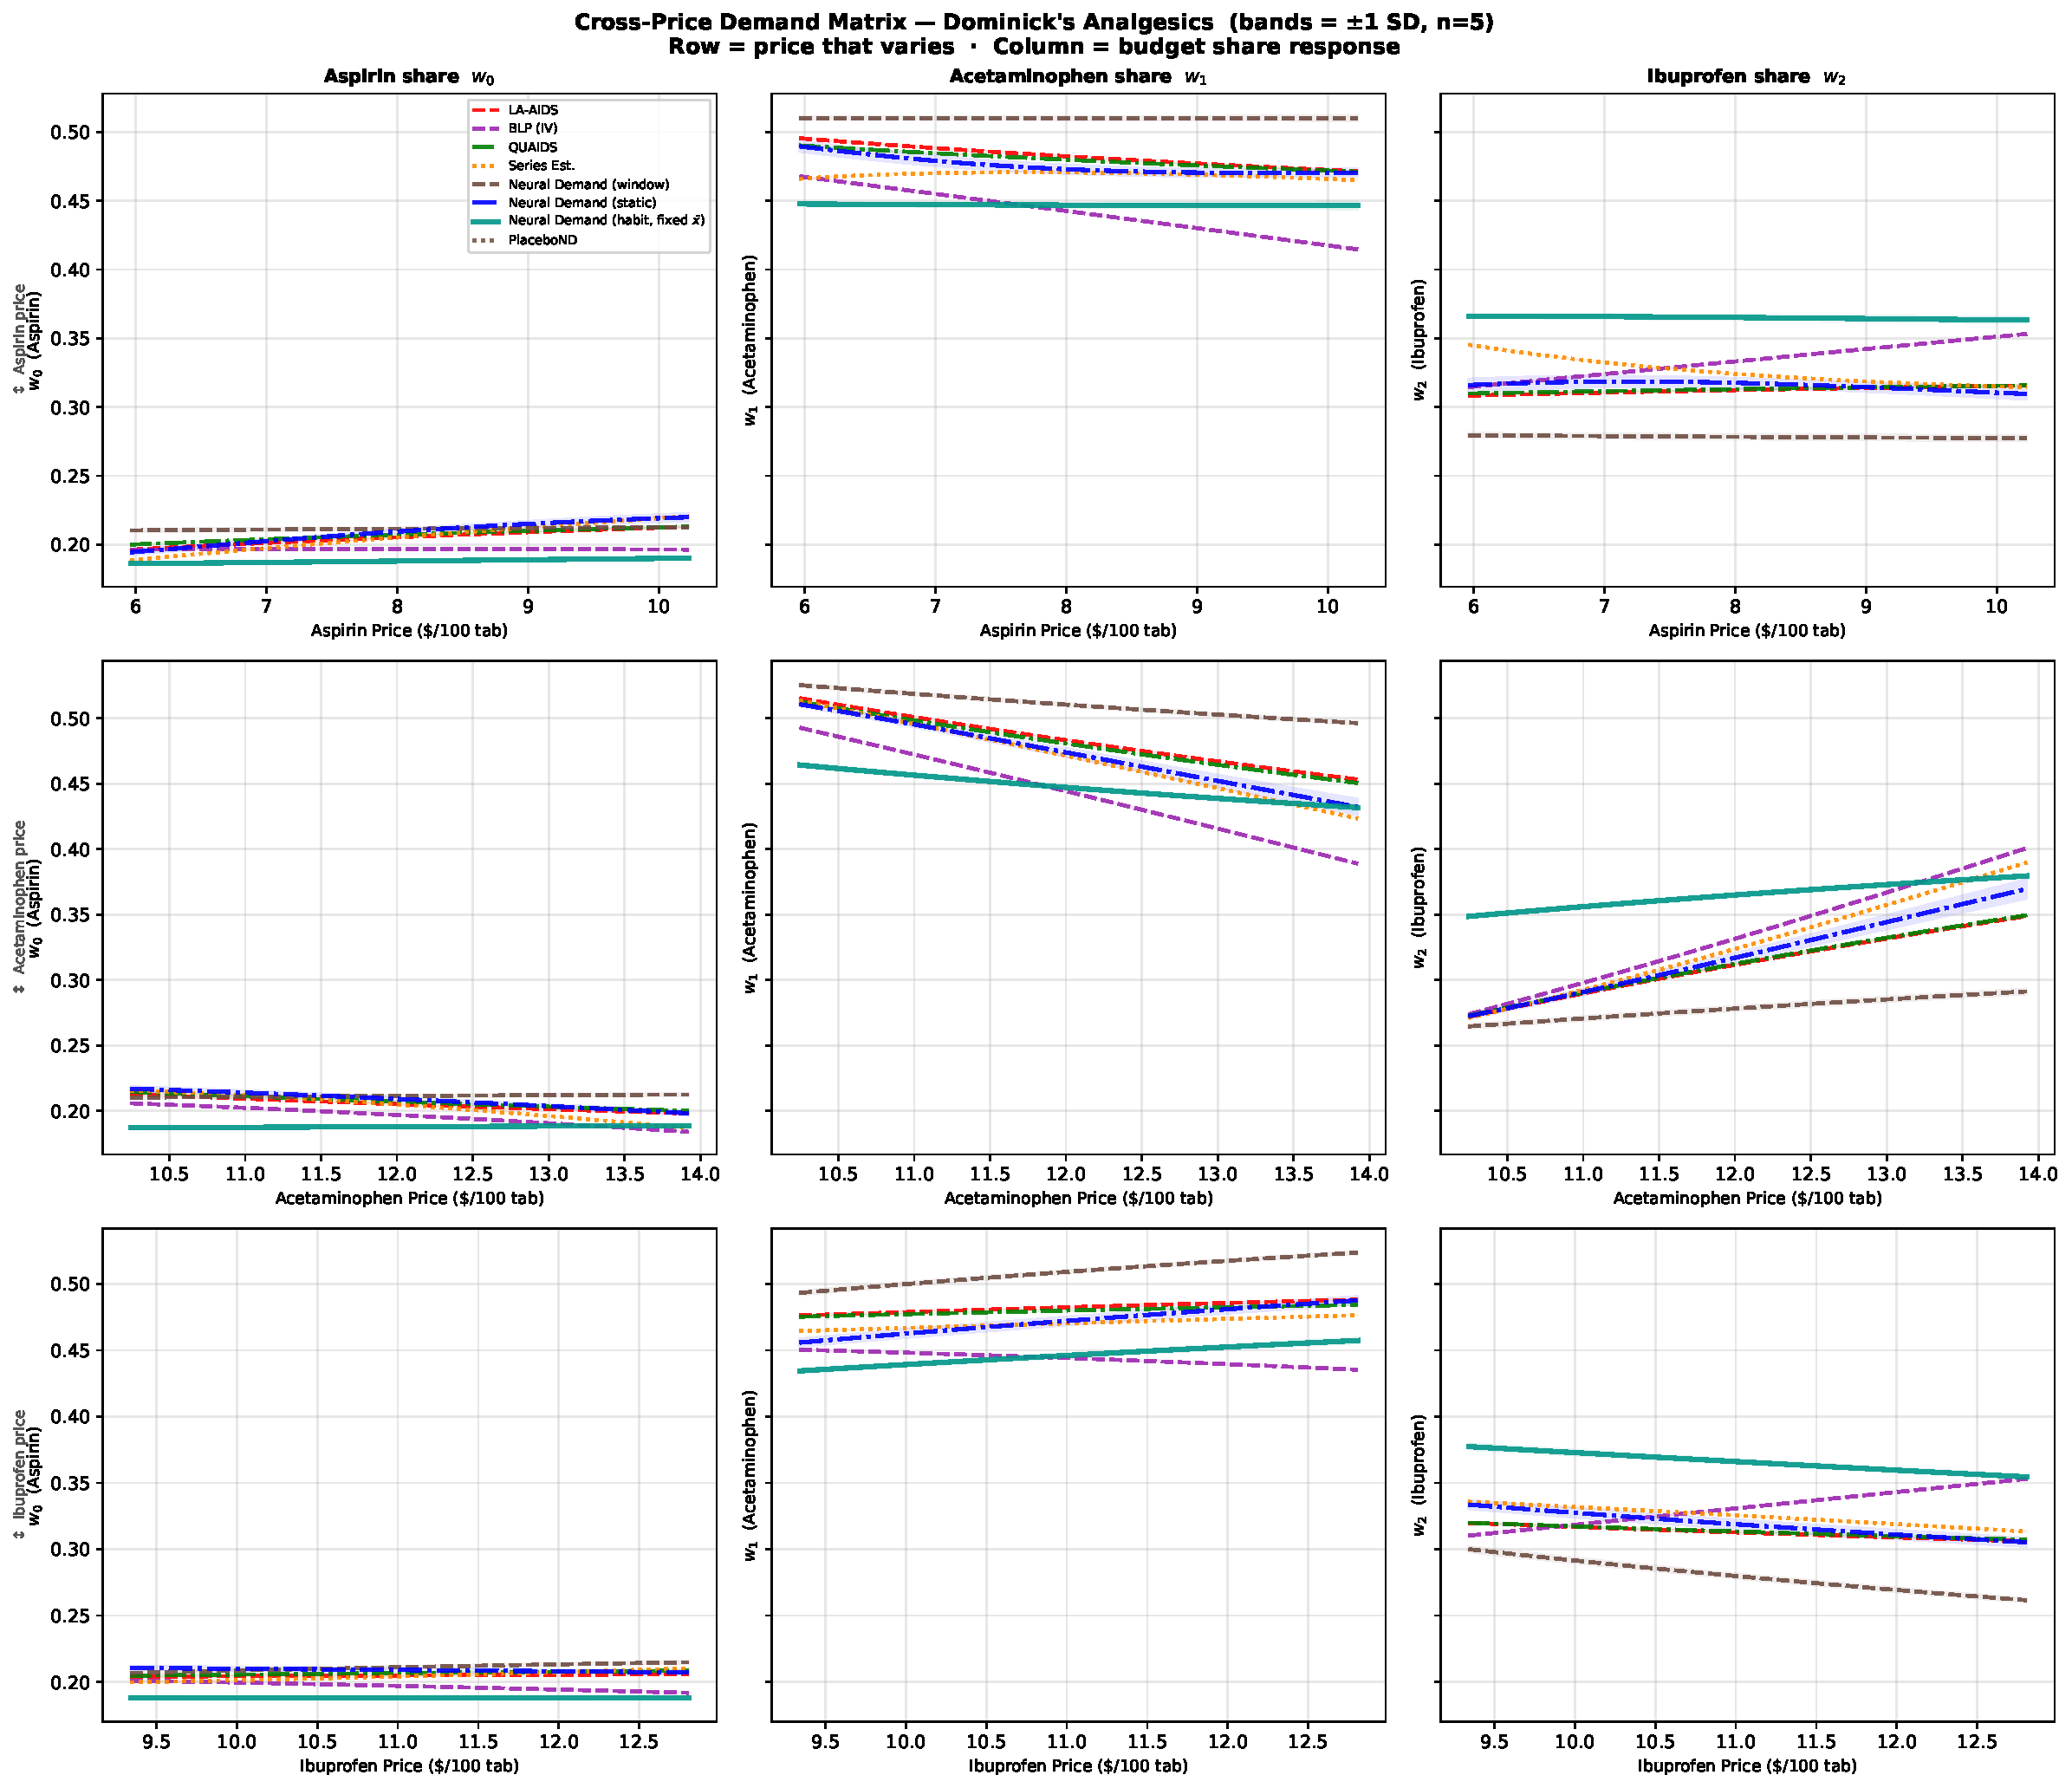
\includegraphics[width=\textwidth]{results/neural_demand/dominicks/figures/fig_mdp_advantage.pdf}
  \caption{Cross-Price Demand Matrix — Dominick's Analgesics. Shaded bands indicate $\pm 1$ standard deviation across 5 independent re-estimations.}
  \label{fig:dom_mdp}
\end{figure}

\begin{figure}[htbp]
  \centering
  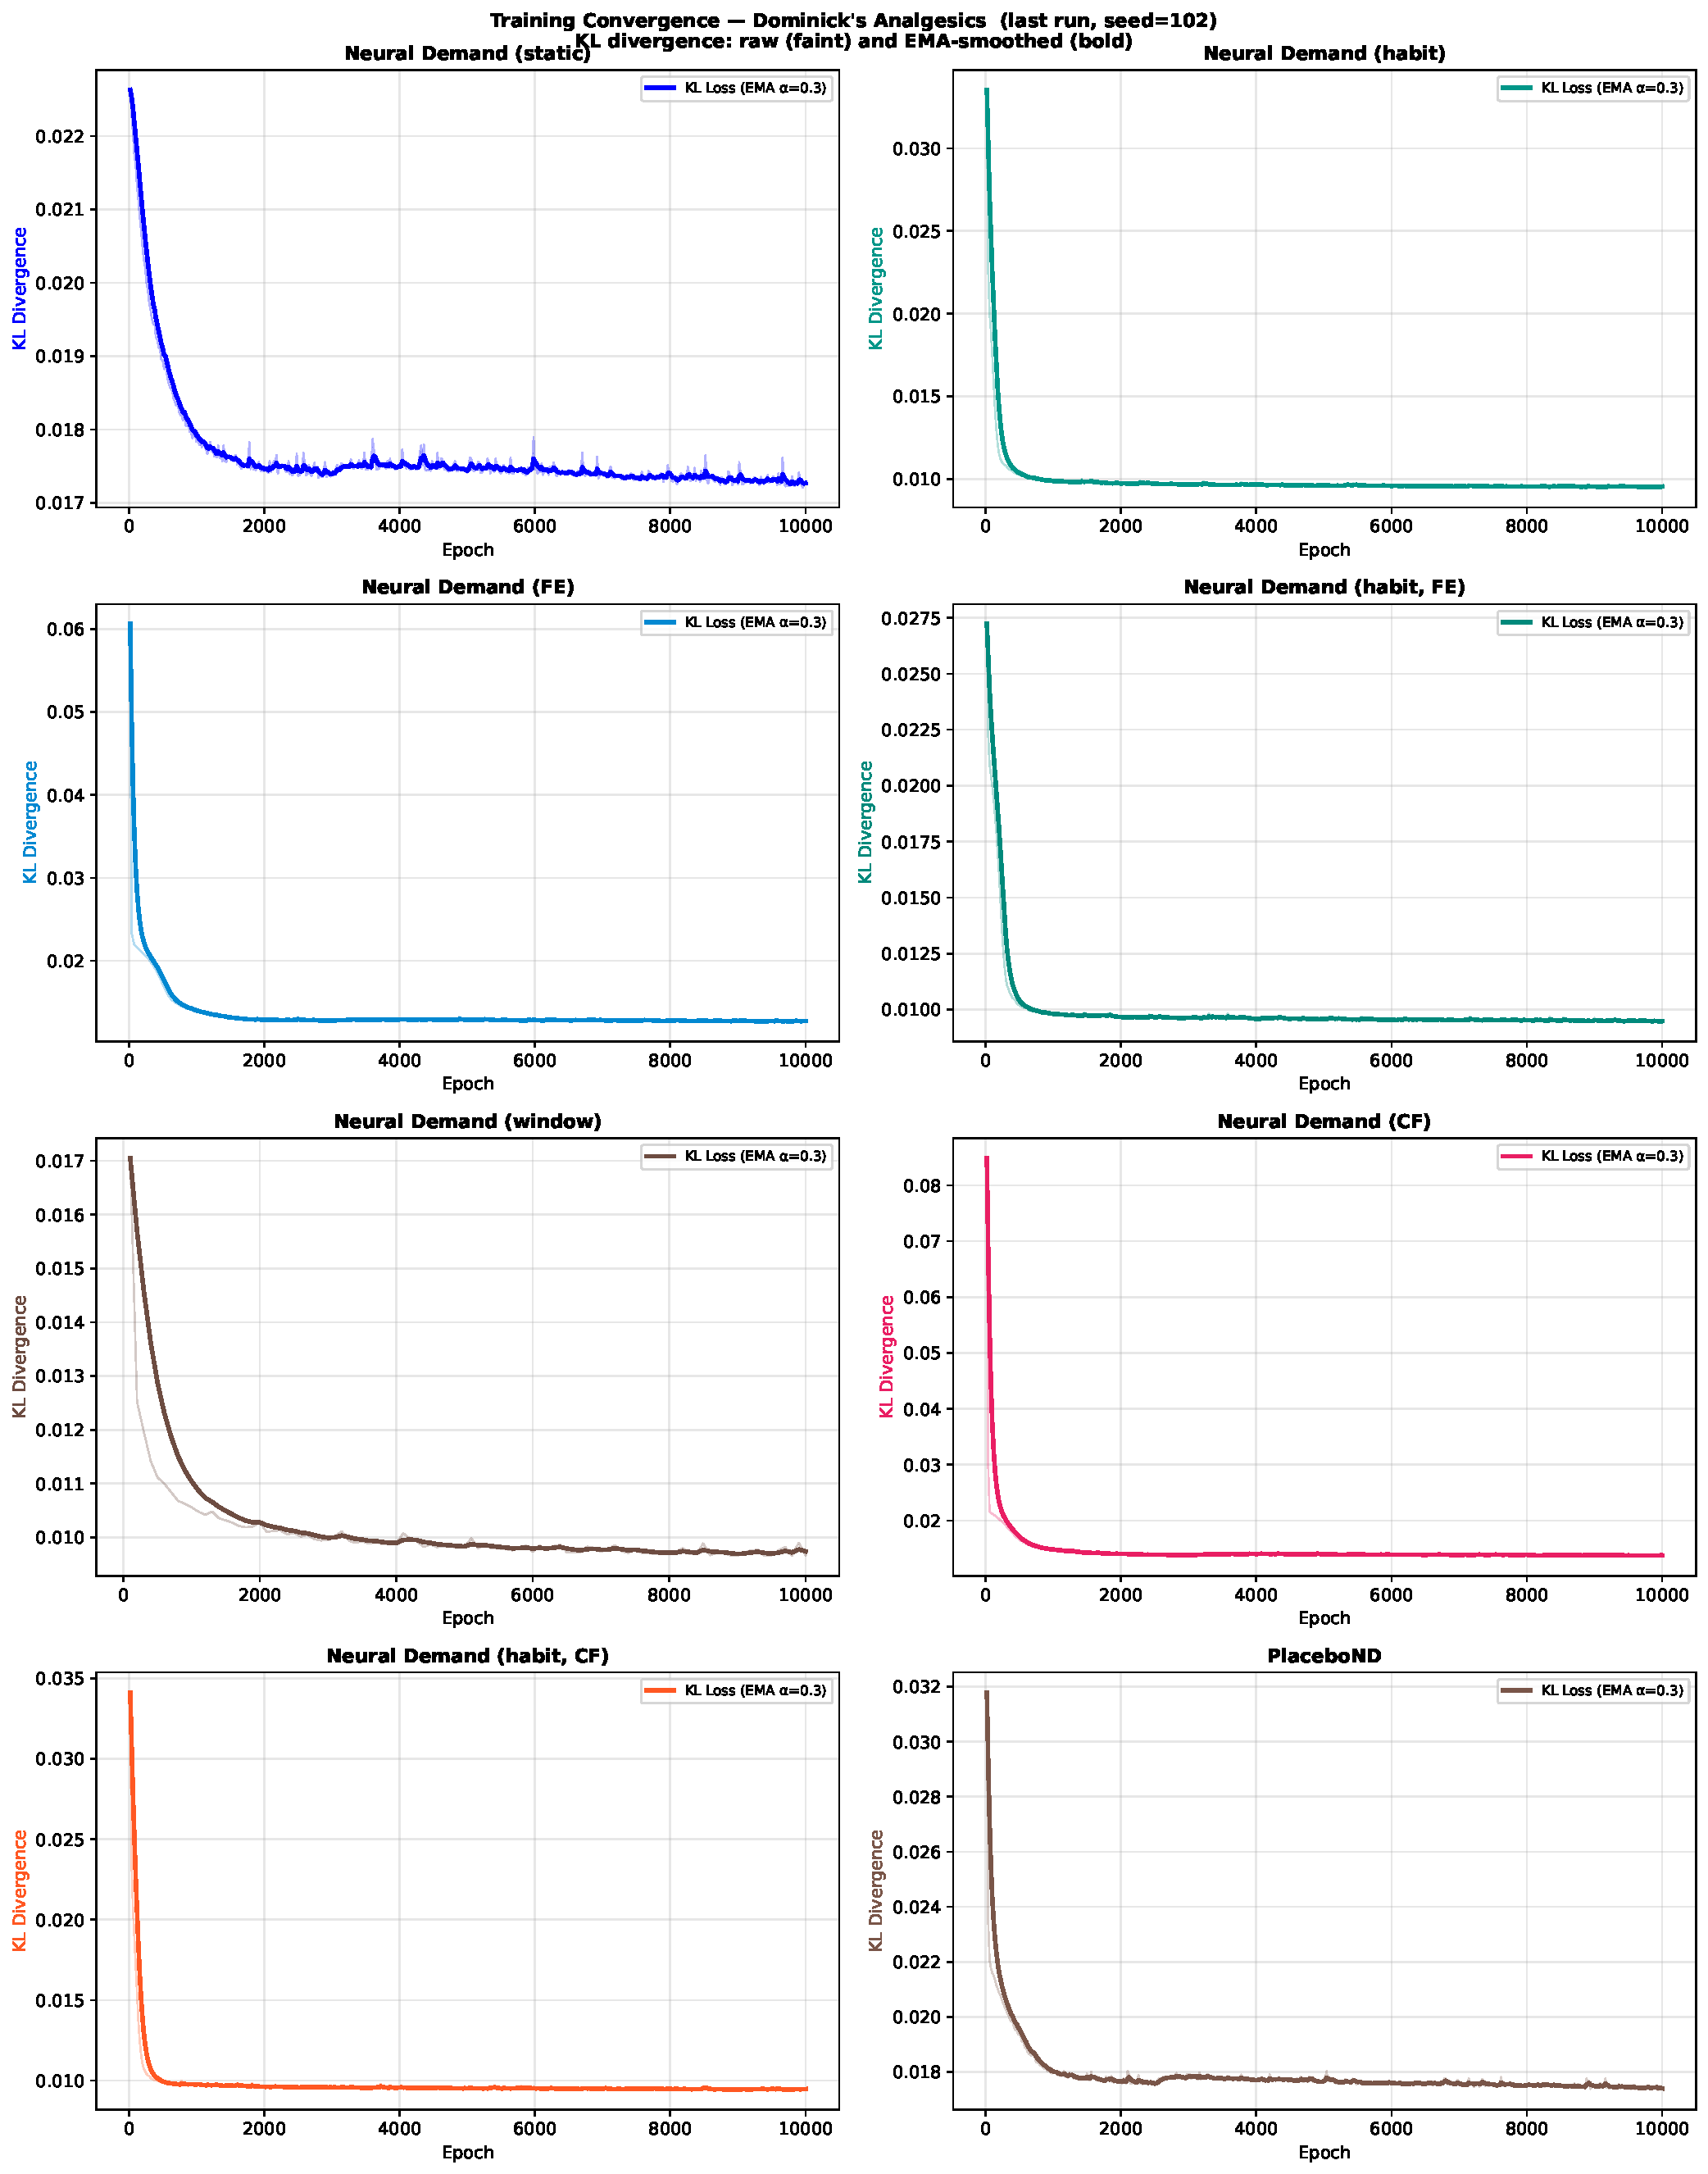
\includegraphics[width=\textwidth]{results/neural_demand/dominicks/figures/fig_convergence.pdf}
  \caption{Training Convergence — Dominick's Analgesics (last run).}
  \label{fig:dom_conv}
\end{figure}

\begin{figure}[htbp]
  \centering
  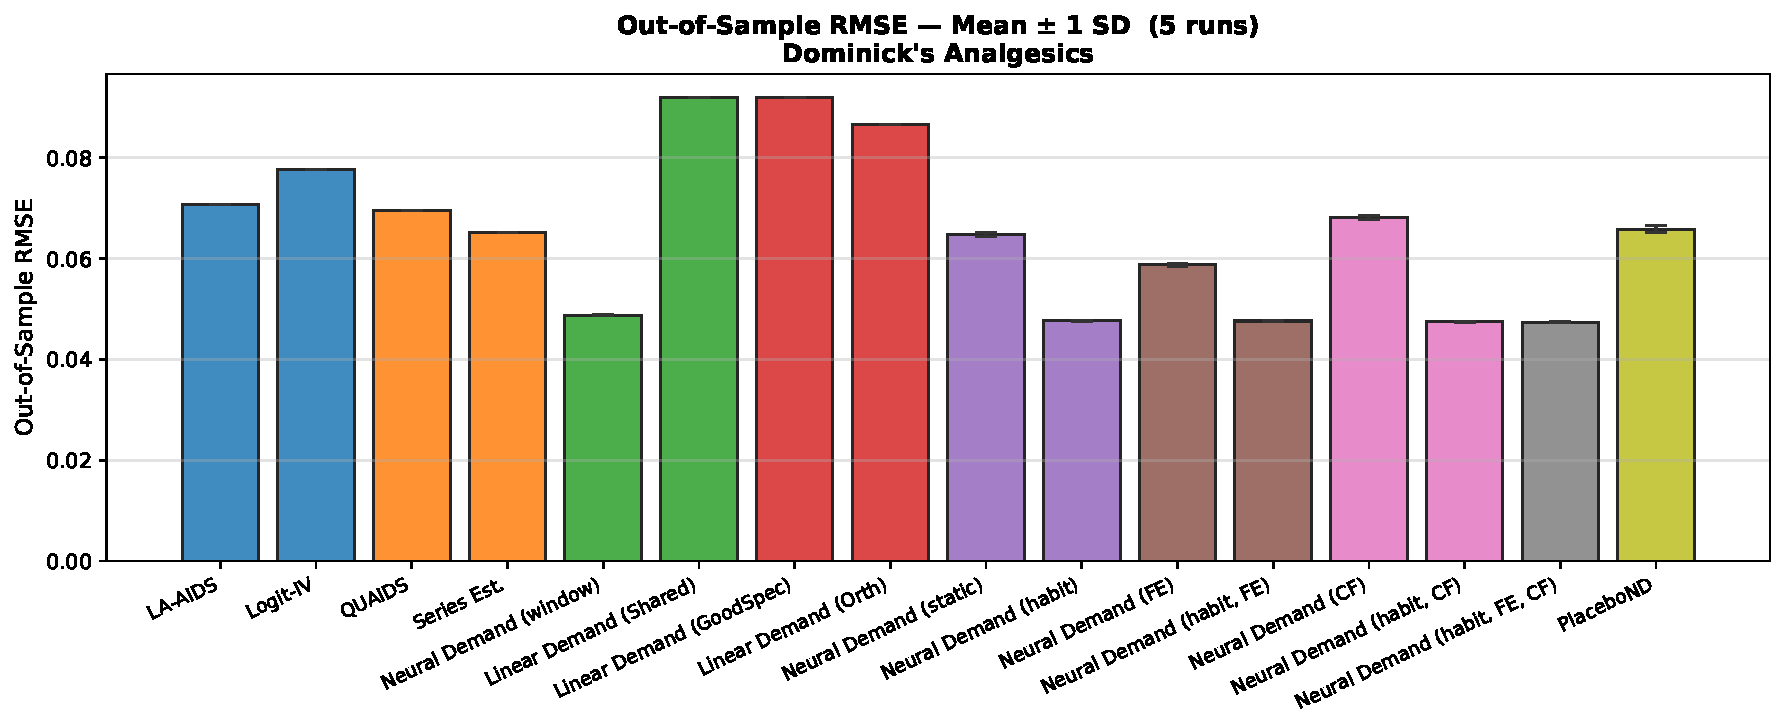
\includegraphics[width=\textwidth]{results/neural_demand/dominicks/figures/fig_rmse_bars.pdf}
  \caption{Out-of-Sample RMSE across all models — mean $\pm 1$ SD over 5 runs.}
  \label{fig:dom_rmse_bars}
\end{figure}

\begin{figure}[htbp]
  \centering
  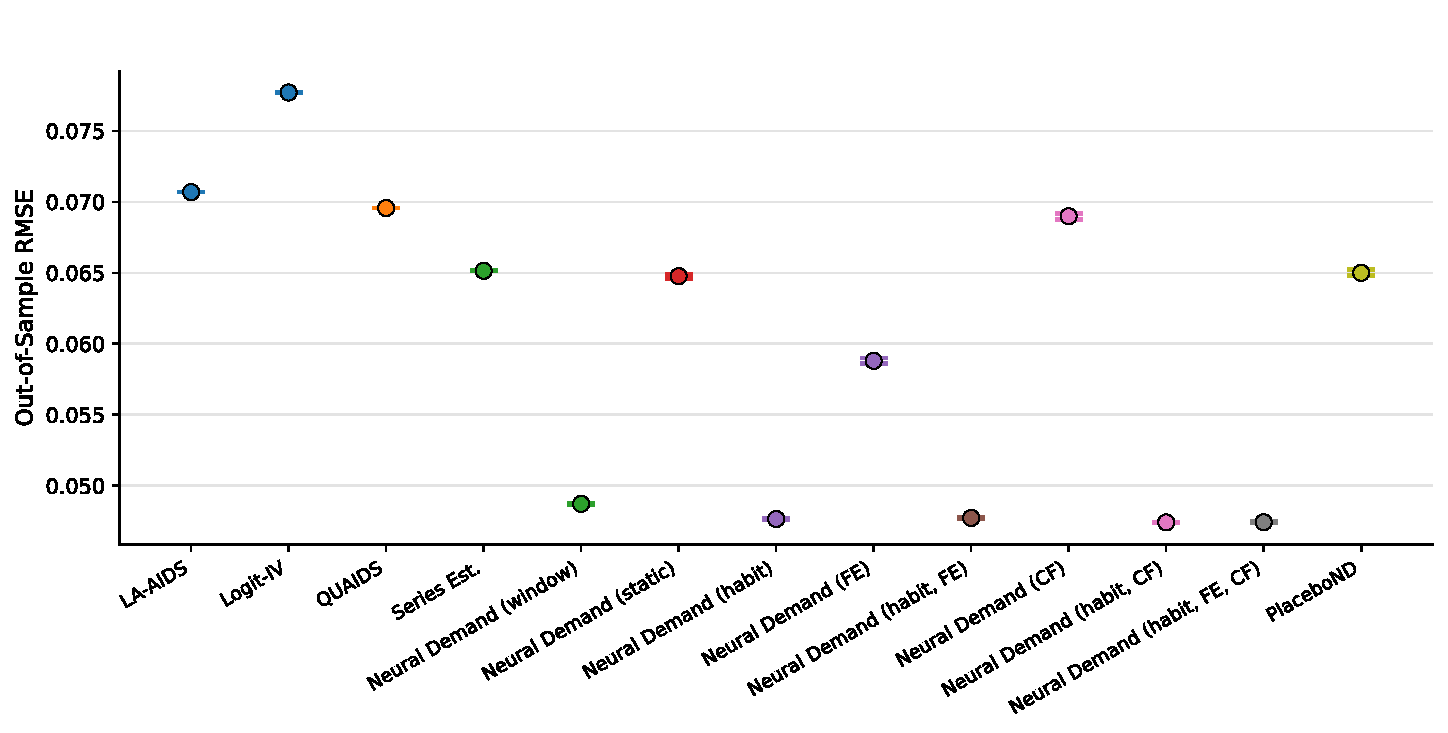
\includegraphics[width=\textwidth]{results/neural_demand/dominicks/figures/fig_rmse_scatter.pdf}
  \caption{Out-of-Sample RMSE across all models — mean $\pm 1$ SE over 5 runs.}
  \label{fig:dom_rmse_scatter}
\end{figure}

\begin{figure}[htbp]
  \centering
  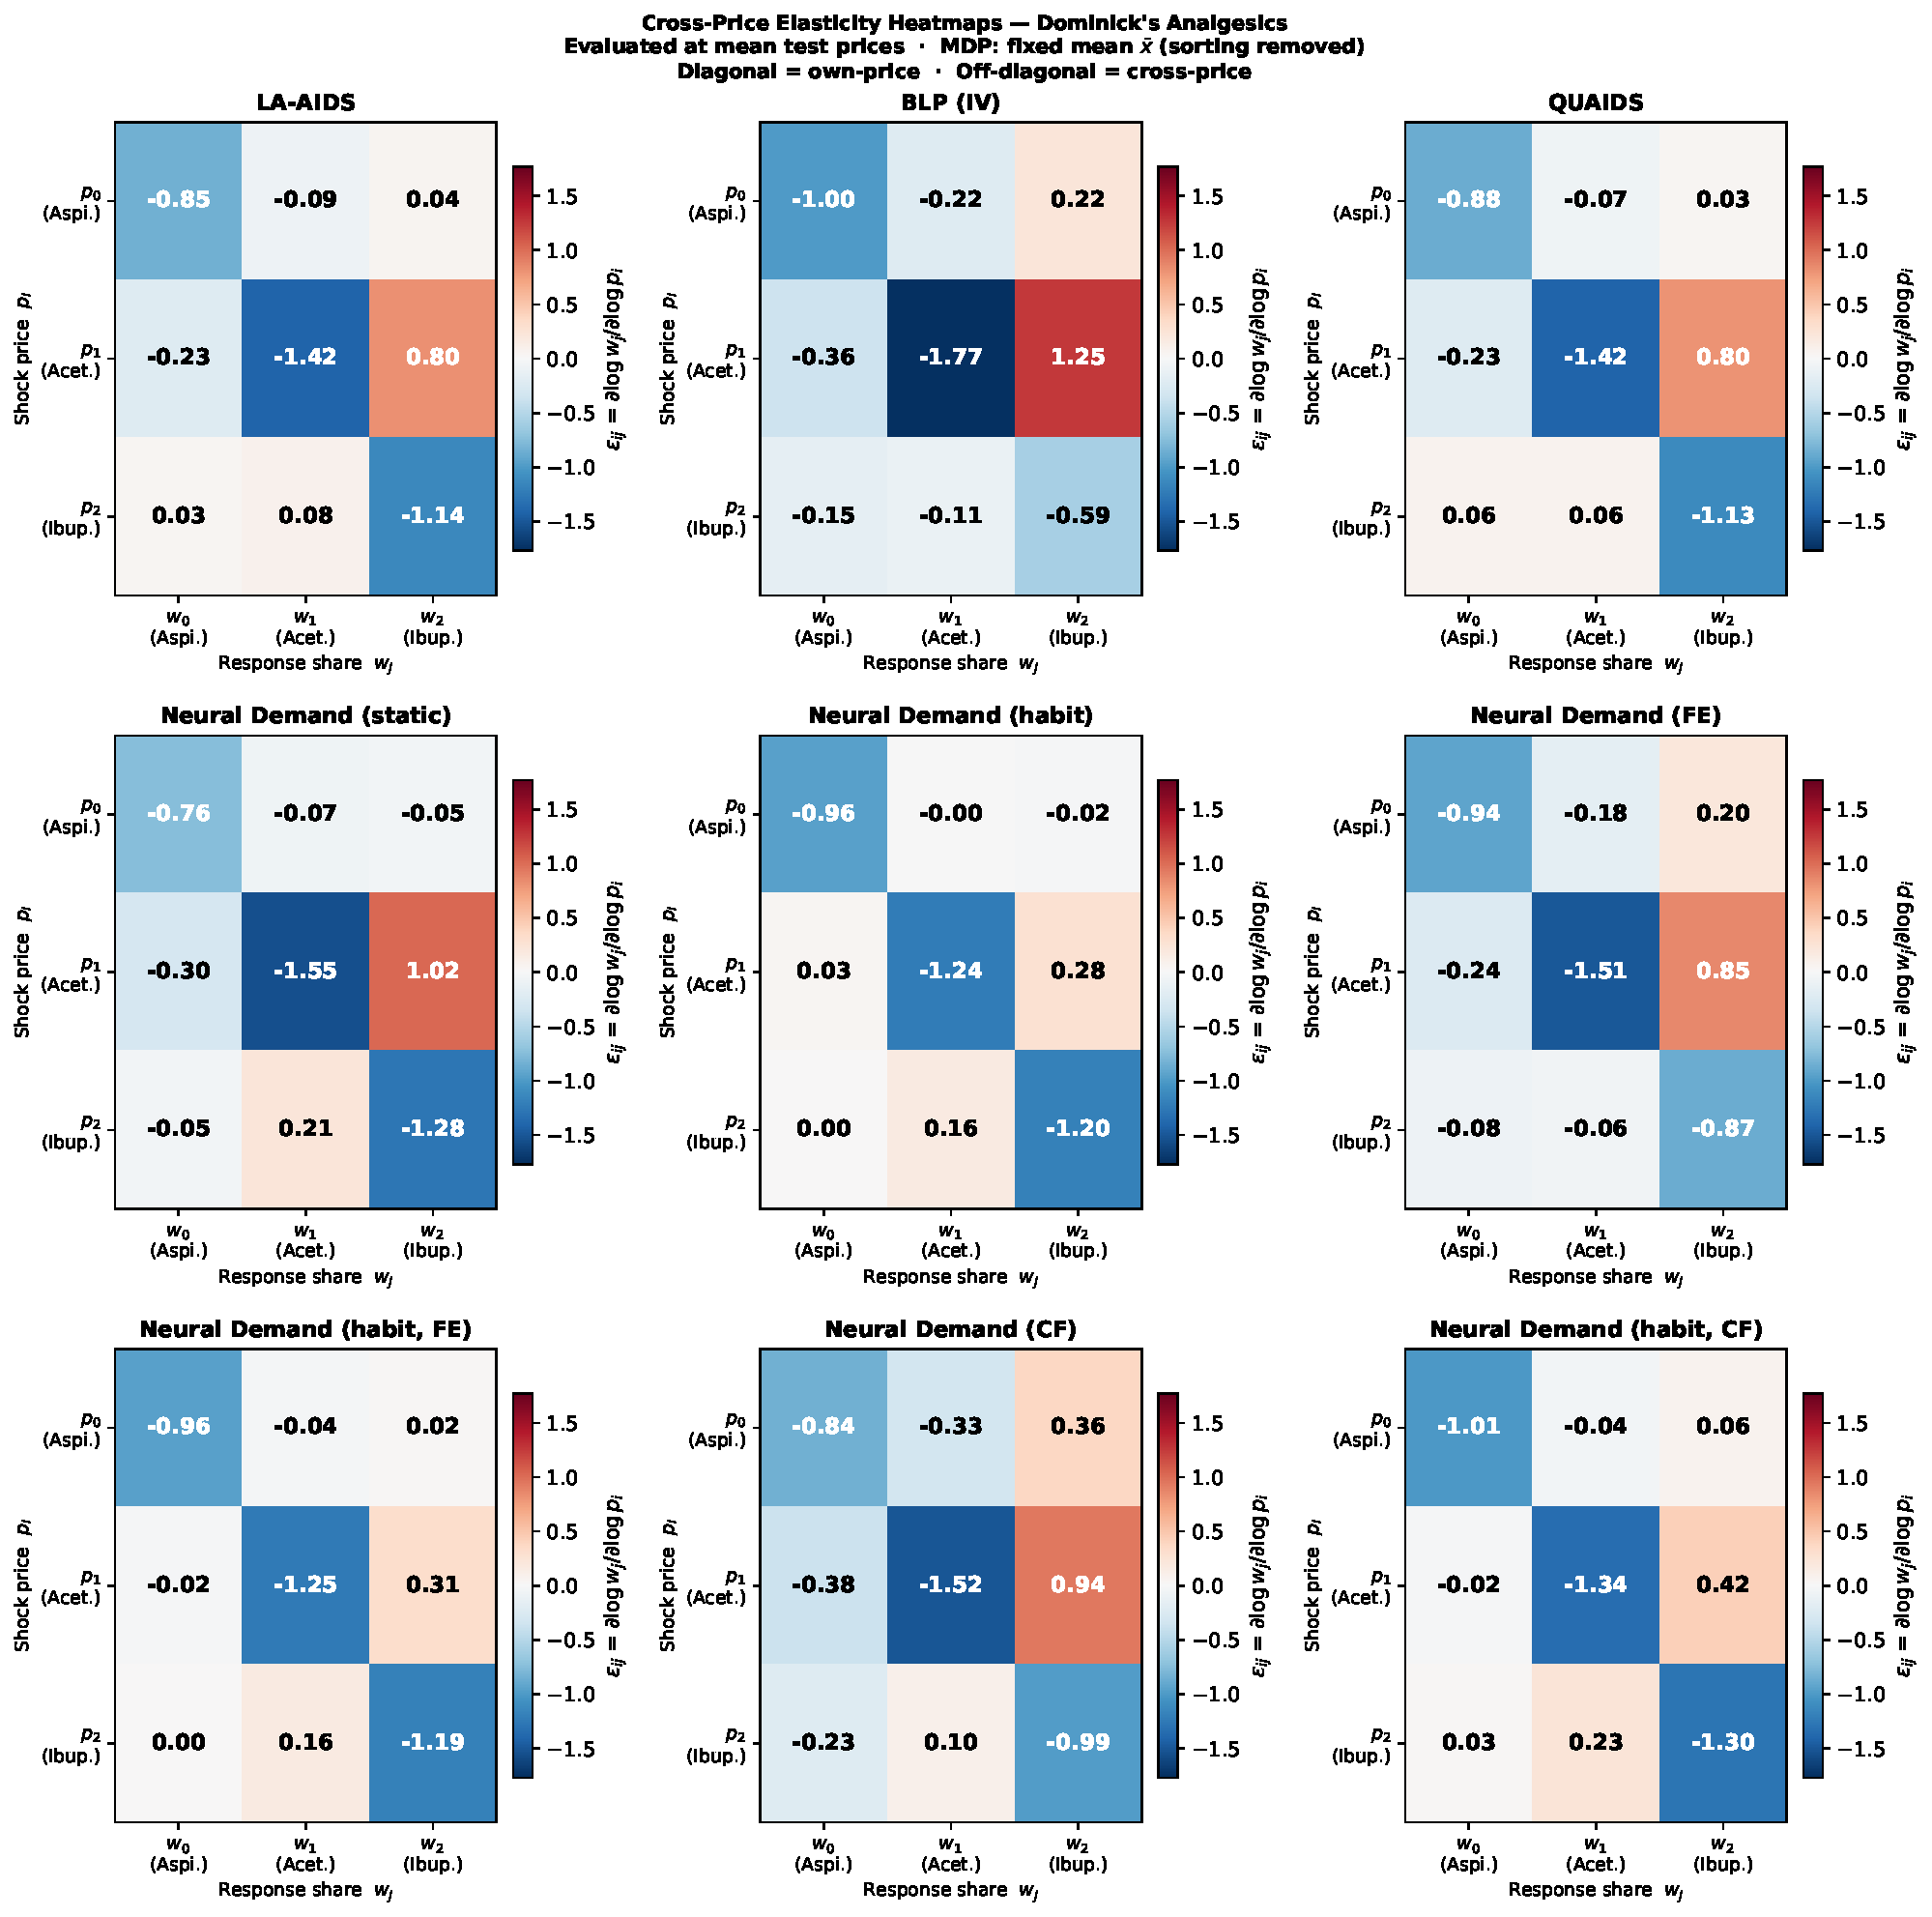
\includegraphics[width=\textwidth]{results/neural_demand/dominicks/figures/fig_cross_elast_heatmap.pdf}
  \caption{Cross-Price Elasticity Heatmaps.}
  \label{fig:dom_cross_elast}
\end{figure}

\begin{figure}[htbp]
  \centering
  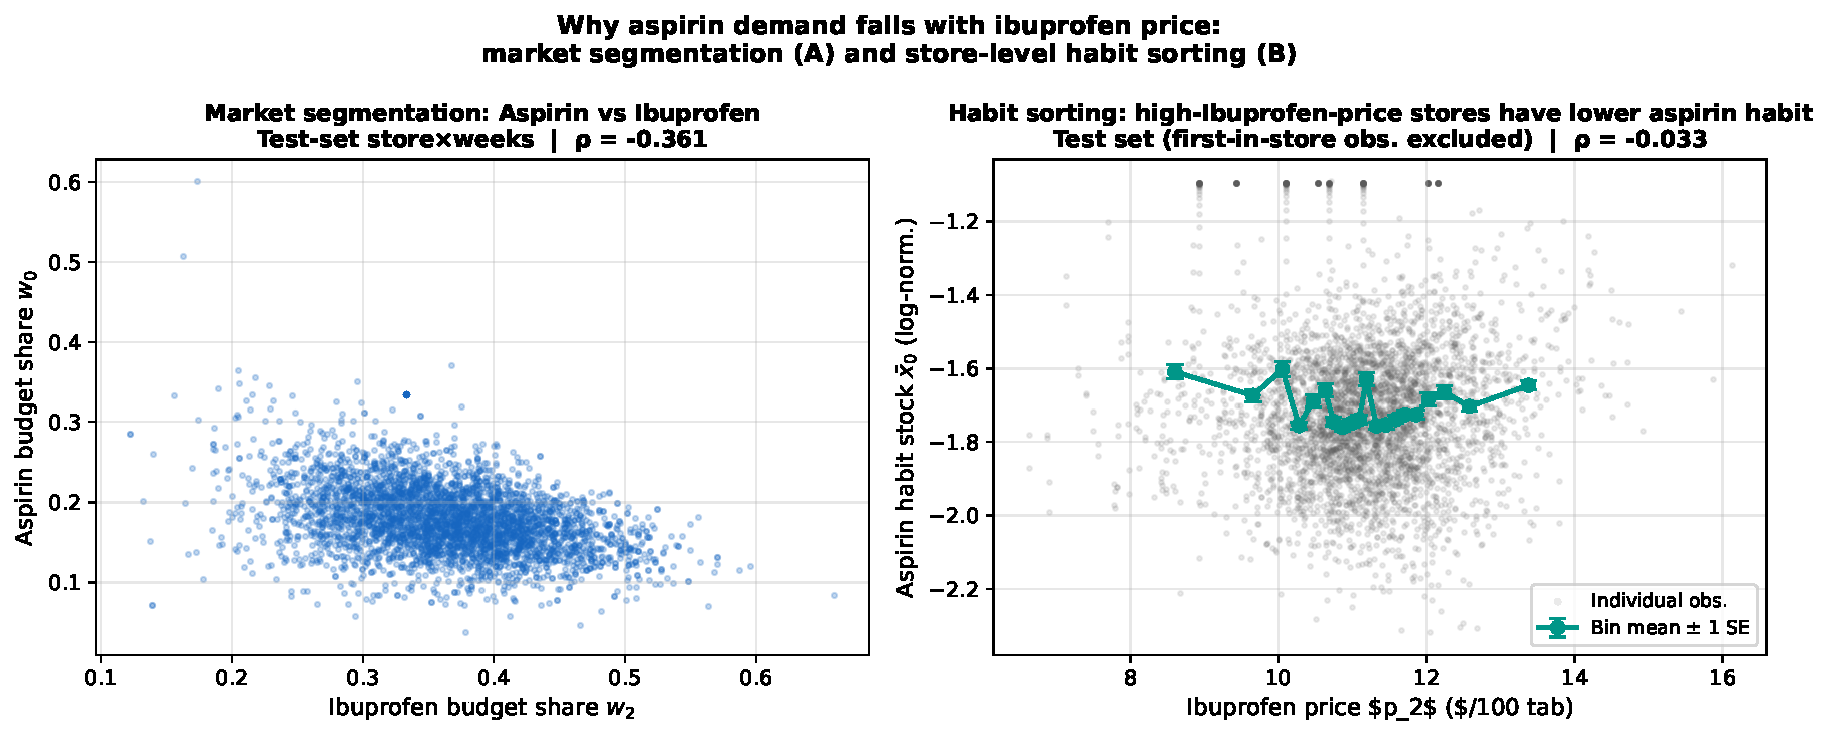
\includegraphics[width=\textwidth]{results/neural_demand/dominicks/figures/fig_segmentation_sorting.pdf}
  \caption{Market segmentation and habit-sorting diagnostics.}
  \label{fig:dom_sorting}
\end{figure}

\begin{figure}[htbp]
  \centering
  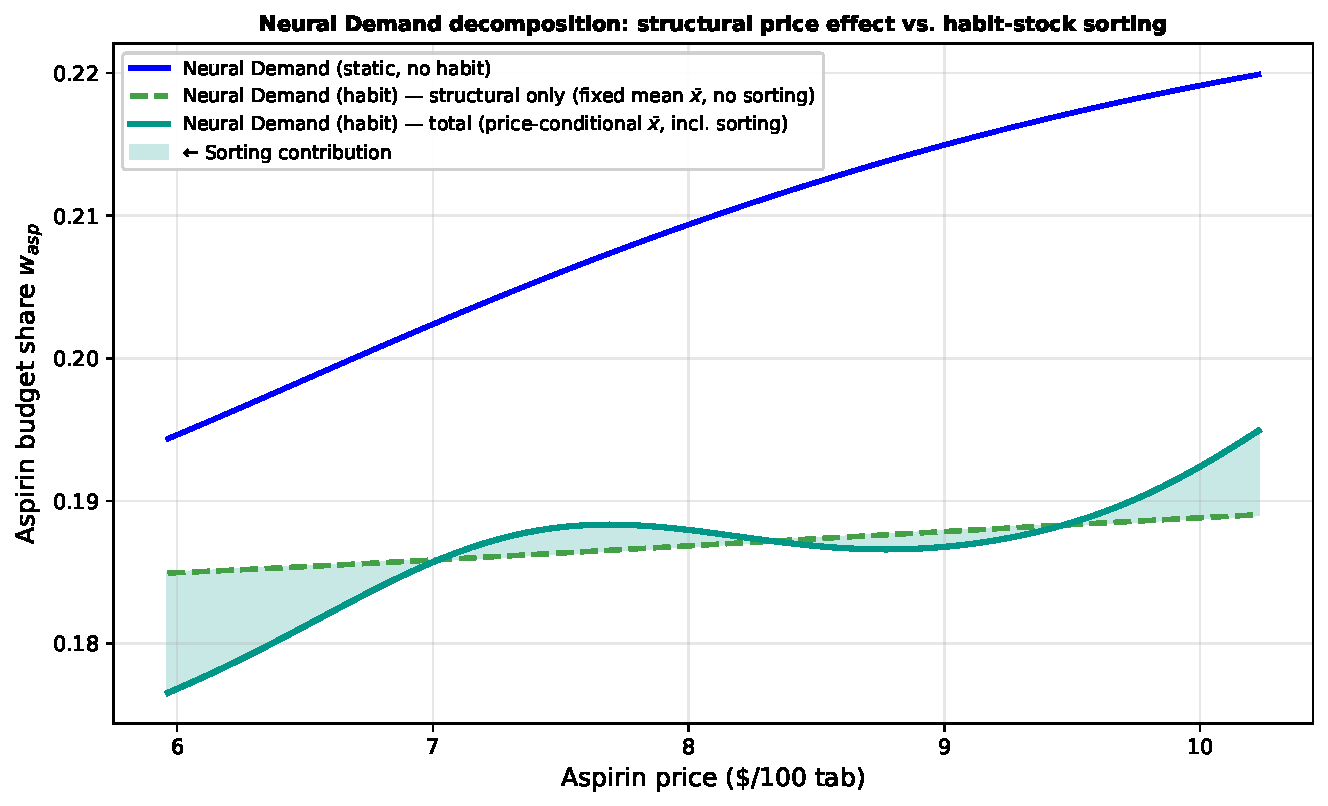
\includegraphics[width=\textwidth]{results/neural_demand/dominicks/figures/fig_mdp_decomposition.pdf}
  \caption{MDP demand decomposition: structural price effect vs. habit-stock sorting.}
  \label{fig:dom_decomp}
\end{figure}
